\documentclass{acm_proc_article-sp}
\bibliographystyle{unsrt}
\usepackage{amssymb,mathtools,graphicx,algorithm,amsmath,algpseudocode}
\begin{document}

\title{Ford-Fulkerson Maximum Flow}
\subtitle{Analysis of Augmenting Paths Techniques}

\numberofauthors{4} 
\author{
\alignauthor
Pedro Rodriguez\\
       \affaddr{University of Colorado at Boulder}\\
       \email{p.rodriguez@colorado.edu}
}

\maketitle
\begin{abstract}
Abstract text. Abstract text. Abstract text. Abstract text. Abstract text. Abstract text. Abstract text. 
\end{abstract}

\section{Introduction}
The first research into network flow algorithms began in the early and mid 20th century. Initial research by A.N. Tolstoi sought to optimize production networks such as railroads in the Soviet Union\cite{Schrijver:2002dj}. The subject later picked up interest amongst the American scientists Ford and Fulkerson who devised the first known algorithm for computing the maximum flow through a network\cite{Ford:1956vc}. 

The maximum flow problem is defined by: Finding the maximum flow through a network from a source vertex $s$ to a sink vertex $t$ in a directed graph $G$ which has edges labeled with flow capacities.

Twenty years after Ford-Fulkerson published their results Edmonds and Karp independently improved upon the algorithm by replacing the depth-first search strategy used in Fork-Fulkerson with breadth-first search\cite{Edmonds:1972ht}. This change improved the algorithmic efficiency from $O(E|f|)$ where $f$ is the maximum flow to $O(VE^2)$. This idea was further improved upon by Dinic's who exploited the property that the flow paths were monotonically increasing to achieve an even better $O(V^2E)$ running time\cite{Dinic:lsM40ti7}. All of these algorithms share a common strategy: find an augmenting path from $s$ to $t$ to push flow across and repeat until there is no such path. At this point the algorithm terminates and returns the maximum flow value and paths.

Beyond the natural applications of maximum flow algorithms to optimizing supply chains, routing, and others it has gained popularity as a sub-algorithm call in more advanced problems. For example, it was recently used to solve the k-clique densest subgraph problem\cite{tsourakakis2015k}, and various computer vision such as object category segmentation, image deconvolution, super resolution, texture restoration, character completion, and 3D segmentation\cite{Verma:2012gs}. It has also been used to solve other problems such as minimum path cover in directed acyclic graphs, maximum cardinality bipartite matching, and in the "real-world" baseball elimination, airline scheduling, and circulation-demand\cite{wiki:maxflow}.

\section{Problem Statement}
\subsection{Formal Problem Statement}
\label{formal-problem-statement}
Now we proceed to formally defining the maximum flow problem. The problem is defined as given a graph with: 
\begin{enumerate}
	\item Vertex set $V$
	\item Directed edge set $E$
	\item Source vertex $s\in V$ such that no edges are incident
	\item Sink vertex $t\in V$ such that no edges leave it
	\item Edge capacities $c_{uv}\in \mathbb{R}^+, \forall (u,v)\in E$
\end{enumerate}

And subject to the conditions:
\begin{enumerate}
	\item $f_{uv}\coloneqq$ variable indicating flow from $u$ to $v$
	\item  $f_{uv}\le c_{uv},\forall (u,v)\in E$
	\item $\forall v\in V\text{ such that }v\ne s,t:\sum_{(u,v)\in E}f_{uv}=\sum_{(v, u)\in E} f_{vu}$
\end{enumerate}

Find the flow assignments $f_{uv}$ such that network flow $|f|\coloneqq\sum_{(s,v)\in E}f_{sv}$ is maximized.

\subsection{Graphical Depiction}
To fix ideas we will continue by describing a concrete instance of the problem. For example, consider the example in figure \ref{simple-flow}\cite{wiki:fordfulk}. In the figure, each edge is labeled by a pair of numbers which are presented as $f_{uv}/c_{uv}$. This represents how much flow $f_{uv}$ is passing through an edge with capacity $c_{uv}$. By inspection, it is easy to deduce that the maximum flow is $2000$ with $1000$ flowing through the top and $1000$ flowing through the bottom. This representation makes the meaning of the conditions (1) and (2) clear. Condition (3) expresses that the flow into any vertex which is not a source or sink must be the flow out of that vertex. Finally, the objective can be explained by noting (with proof later) that the maximum flow from $A$ to $D$ is equivalent to taking a cut across $A$.

Before moving on, lets consider a simple algorithm: find a path through the network and push the maximum possible flow through until pushing flow is impossible. One can see this may result in the optimal solution, but if one path found is the one cross $BC$, then the optimal flow will never be found. This hints that the simple graph construction is insufficient to solve the maximum flow problem.

\begin{figure}[!ht]
	\caption{Simple flow network}
	\centering
	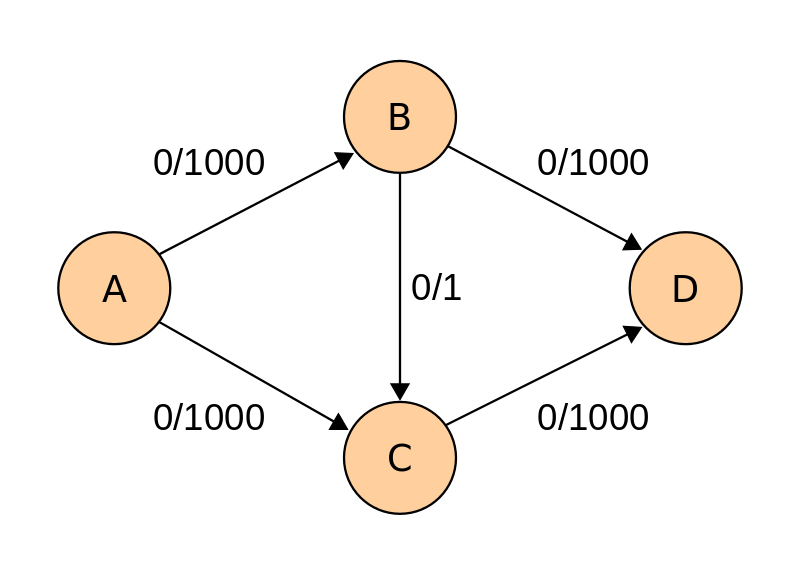
\includegraphics[width=0.4\textwidth]{images/simple-flow.png}
	\label{simple-flow}
\end{figure}

\section{Algorithm Analysis}
In this section we will first present the very similar Ford-Fulkerson and Edmonds-Karp algorithms, prove their correctness, and analyze their asymptotic behavior in both time and space complexity.

\subsection{Algorithm}
Before proceeding to the algorithm itself, we must make a few additional definitions and constructions. First we will define a $G_f(V,E_f)$ which we will call the residual graph. In this graph, the capacities are defined as $c^f_{uv}=c_{uv}-f_{uv}$ and there is zero flow. We additionally define that $\forall (u,v)\in E f_{uv}=-f_{vu}$. Combining these two loosens the constraints from the original graph to allow cases where if $f_{uv}>0$ and $c_{uv}=0$ that $c^f_{vu}=c_{vu}-f_{vu}=f_{uv}>0$. As will be proven, this allows for algorithm to function correctly. We now proceed to stating the main algorithm as Algorithm \ref{ff-ek-algorithm}.

\begin{algorithm}
\label{ff-ek-algorithm}
\caption{Ford-Fulkerson and Edmonds-Karp}
\begin{algorithmic}[1]
\Function{max\_flow(G,c,s,t)}{}
\State Input: $G,c,s,t$ as described in \ref{formal-problem-statement}
\State Output: Flow $f_{max}$ and paths to achieve it
\Loop
\State $path\gets augmenting\_path(G_f,s,t)$
\If {$path = None$}
\State break
\EndIf
\State $f_{min}=\min_{(u,v)\in path} c^f_{uv}$
\For{$(u,v)\in path$}
\State $f_{uv}\gets f_{uv}+f_{min}$
\State $f_{vu}\gets f_{vu}-f_{min}$
\EndFor
\EndLoop
\State $f_{max}\gets \sum_{(s,v)\in E}f_{sv}$
\State $paths\gets$ paths/flows from $s$ to $t$ in created graph
\State \Return $f_{max},paths$
\EndFunction
\end{algorithmic}
\end{algorithm}

The algorithm proceeds in two alternating phases: finding an augmenting path from $s$ to $t$ in $G_f$ and pushing the maximal viable flow across that path. When an augmenting path cannot be found, then the algorithm terminates and returns the current maximal flow.

We define an augmenting path as any path from $s$ to $t$ in $G_f$ such that $c^f_{uv}>0\ \forall (u,v)\in path$. The algorithm was not previously specified because its definition determines whether the algorithm is known as Ford-Fulkerson or Edmonds-Karp. If the augmenting path is found using depth first search then the algorithm is called Fork-Fulkerson. If the augmenting path is found using breadth first search then the algorithm is called Edmonds-Karp. With that in mind, we now define the two possible augmenting path algorithms. Note that the $0th$ element of a list is considered the back and the last element of a list is considered the front. Additionally the notation $vec[a;b]$ is short for creating a vector of length $b$ with values initialized to $a$.

\begin{algorithm}
\begin{algorithmic}[1]
\label{ap-algorithm}
\Function{augmenting\_path($G_f$, s, t, search)}{}
\State $V, E_f\gets G_f$
\State $search\_list \gets list()$
\If {$search = BFS$}
\State $pop \gets list.pop\_front$
\State $push \gets list.push\_back$
\Else
\State $pop \gets list.pop\_front$
\State $push \gets list.push\_front$
\EndIf
\State $push(search\_list, s)$
\State $distances\gets vec[\infty; |V|]$
\State $parents\gets vec[\infty; |V|]$
\State $u\gets pop(search\_list)$
\While{$u \ne None\ and\ u\ne t$}
\For{$v$ in $neighbors(u)$}
\If{$distances[v] =\infty\ and\ c^f_{uv}>0$}
\State $distances[v]\gets distances[u] + 1$
\State $parents[v]\gets u$
\State $push(search\_list, v)$
\EndIf
\EndFor
\State $u\gets pop(search\_list)$
\EndWhile
\State\Return $u == t$, reconstruct\_path(s, t, parents)
\EndFunction
\Statex
\Function{reconstruct\_path(s, t, parents)}{}
\State $path\gets list()$
\State $node\gets t$
\Loop
\State $path.append(node)$
\If{$node == s$}
\State \textbf{break}
\EndIf
\State $path\gets parents[node]$
\EndLoop
\State\Return $reverse(path)$
\EndFunction
\end{algorithmic}
\end{algorithm}


\bibliographystyle{abbrv}
\bibliography{references}

%\balancecolumns 

\end{document}
